\documentclass[letterpaper,11pt,twocolumn]{article}
\usepackage[T1]{fontenc}
\usepackage[utf8]{inputenc}
\usepackage{lmodern}
\usepackage{amsmath}
\usepackage{amsfonts}
\usepackage{amssymb}
\usepackage{amsthm}
\usepackage{float}
\usepackage{graphicx}
\usepackage{caption}
\usepackage{subcaption}
\usepackage{color}
\usepackage{xcolor}
\usepackage{url}
\usepackage{textcomp}
\usepackage{listings}
\usepackage{hyperref}
\usepackage{parskip}
\usepackage{todonotes}
\usepackage[
backend=biber,
style=alphabetic,
]{biblatex}
\usepackage{csquotes}
\setlength{\marginparwidth}{2cm}
\usepackage[inline]{enumitem}
\newlist{inlinelist}{enumerate*}{1}
\setlist[inlinelist]{label=(\roman*)}

\addbibresource{philo.bib}

\title{What Radical Behaviorism is to modern AI analysis}
\author{Paolo Marzolo}
\date{\today}

\begin{document}
\twocolumn[
    \begin{@twocolumnfalse}
        \maketitle
        %\tableofcontents
        \begin{abstract}
            Artificial Intelligence powered machines are being increasingly relied upon in all facets of human life. As these machines and their ecosystems grow more complex, equally powerful systems for interpreting, analyzing and predicting their behavior are needed. This raises the need for new, interdisciplinary research to expand upon computer science incorporating insights from other sciences. Here, I explore the philosophical background of Behavioral Science as formulated by B.F. Skinner, and the insights it can give practitioners of Artificial Intelligence when applied to machine behavior.
        \end{abstract}
    \end{@twocolumnfalse}
    \medskip
]

\section*{Introduction}
Recent advancements in Artificial Intelligence (most notably Natural Language Processing) have driven state-of-the-art models to extremely complex models. This is a core feature of the models:
\begin{inlinelist}
    \item progress on Deep Learning is strongly reliant on it\cite{thompsonComputationalLimitsDeep2022},
    \item the CEO of OpenAI (the company behind ChatGPT) Sam Altman proposed the "amount of compute" as a possible starting point for legislative licensing efforts,
    \item for Natural Language Processing, it is in the name itself (Large Language Models, or LLMs).
\end{inlinelist}
With this explosive growth, the difficulty of explaining the behavior of a model has grown to an entire field of study. In the eloquent words of one of the historical papers on the subject, \enquote{if
    you open them up and peer inside, all you can see is a big pile of goo}\cite{mozerUsingRelevanceReduce1989a}.
\todo[inline]{Add a few more words about why single machine and current efforts}
In \cite{rahwanMachineBehaviour2019}, the authors identify 4 levels of scale:
\begin{description}
    \item[single machine]
    \item[collective machine]
    \item[hybrid]
    \item[machines shape]
\end{description}

I focus on using Behavior Analysis as a method of investigating the various levels of scale of machine behavior. After reviewing the main characteristics of Behavior Analysis, I will consider its philosophical background, identified with Radical Behaviorism, highlighting the effect of this philosophical framework on the practice. Lastly, I will propose considering an AI agent as part of a human-AI interaction, and evaluate how the assumption of Radical Behaviorism will impact our conceptualization of the agent, verifying its compatibility with the theory.

% \begin{flushright}
%     One does not simply follow behaviorism.\\
%     \textit{Nobody (2023)}
% \end{flushright}

As any doctrine which lasts long enough, Behaviorism has grown to many variants: even Wikipedia mentions seven\cite{Behaviorism2023}, while a recent review identifies 8\cite{araibaCurrentDiversificationBehaviorism2020}. In this article, I will focus on Radical Behaviorism, developed and championed by B.F. Skinner and later adapted and adopted by different scholars. I will outline the general features of Behaviorism in the next two paragraphs. Although \enquote{Behaviorism is not the science of human behavior; it is the philosophy of that science (page 1, line 1)}\cite{skinnerBehaviorism1976}, such philosophy, still, is tied to the science of human behavior, so some exploration of it will be necessary.

\section*{Behaviorism}
The term "Behaviorism" was coined by J. Watson in 1913\cite{maloneDidJohnWatson2014}, as he incorporated earlier studies on reflexes by Pavlov in a general theory of behavior. Watson argued that psychology needed to focus on behavior, instead on the study of mind, consciousness and introspective methods. Watson was also the first prominent psychologist to argue for psychology as a natural science; this position was later supported by Radical Behaviorism, the philosophy of that science. Around the same time, similar experimental studies were being conducted by Thorndike. These studies formed the basis of the experimental analysis of behavior, further formalized in Skinner's doctoral thesis \cite{skinnerBehaviorOrganismsExperimental1999}. Ultimately, this experimental analysis led to a more practically oriented branch, Applied Behavior Analysis, which has been applied in many behavior domains successfully\cite{wlABABehaviorScience2022}.
Thus, three distinct branches were formed:
\begin{description}
    \item[Behavior Analysis] The experiment based, laboratory-focused discipline which discovered and studies the basic principles behind organisms' behavior.
    \item[Applied Behavior Analysis] The discipline which aims to apply the basic principles behind behavior discovered in laboratory-based experiments to real-world, practical applications, to \enquote*{support positive change in socially important behaviors using basic learning principles}.
    \item[Radical Behaviorism] The philosophy of the Science of Behavior, or Behavior Analysis, is called Radical Behaviorism. It was developed by Skinner\cite{schneiderHistoryTermRadical1987}.
\end{description}

I will now give a brief overview of the first two, then consider how the philosophy affects the science direction and why such a perspective is relevant for AI research.

\subsection*{Behavior Analysis}
Pavlov's experiments identified \textit{classical conditioning}: the process in which a specific stimulus (e.g. a sound) is presented with a stimulus (e.g. food) that already elicits a response (salivation) to pair the response with the first stimulus\cite{iClassicalConditioning2023}. The latter formalization by Skinner drew a distinction between classical conditioning and what he called operant conditioning, a learning process in which modifications to operants (behaviors that \textit{operate} on the environment) are elicited by specific consequences, respectively called reinforcers or punishments if they increase or decrease the probability of reoccurrence of the operant. This forms the basic "three-term contingency": \textit{discriminative stimuli} signal the availability of \textit{reinforcement or punishment} based on a \textit{behavioral response}. Behavior Analysis (more specifically: Skinner) uses these basic principles to explain behavior: actions are behavior, speech is verbal behavior (and to be analyzed as such), thoughts are covert behavior (\enquote{Thinking is behaving (page 66)}\cite{skinnerBehaviorism1976}), social interactions are organisms behaving and providing consequences to each other.\todo{citation?}\todo{say why i said this?}

\subsection*{Applied Behavior Analysis}
Applied Behavior Analysis takes Behavior Analysis out of the laboratory and focuses on achieving change in the real world:
\begin{displayquote}
    Applied behavior analysis, or ABA, is a scientific approach for discovering environmental variables that reliably influence socially significant behavior and for developing a technology of behavior change that takes practical advantage of those discoveries.
    \cite{cooperAppliedBehaviorAnalysis2020}
\end{displayquote}
% The same book notes how the seven\footnote{text} dimensions given by Baer and colleagues in 1987\cite{baerSTILLCURRENTDIMENSIONSAPPLIED1987} are still \enquote*{useful and relevant signposts} to identify ABA research.
Although the specific operations of this branch are out of scope for this article, it is relevant to note that the philosophical background of ABA directly influences ABA practitioners.

\subsection*{Radical Behaviorism}
As stated, Radical Behaviorism is the philosophy of the science of behavior. It is the foundation against which both Experimental Behavior Analysis and Applied Behavior Analysis measure themselves, and what gives direction to the entire field\footnote{Radical Behaviorism is not the only possible Behaviorism, nor is it the most recent. Nonetheless, it is one of the most studied, and it refers to a single author (Skinner), so it is our object of study here.}. The basic tenet of Behaviorism is that \enquote*{A science of behavior is possible}(page 3, \cite{baumUnderstandingBehaviorismBehavior2017}). In addition, it should be considered a \textit{natural} science\cite{baumWhatRadicalBehaviorism2011}\cite{chiesaRadicalBehaviorismPhilosophy1994}(page 179). This results in a relevant distinction from previous psychological approaches: behavioral event do not need any \textit{agent}, as they are not done, but \enquote*{are to be explained by other natural events}\cite{baumWhatRadicalBehaviorism2011}.
A recent review\cite{araibaCurrentDiversificationBehaviorism2020} of Behaviorism currents used the approach to the agent problem as the turning point\todo{wrong word} between them.

Then, as natural events, should they be explained in terms of biology, chemistry, and physics? It is a possibility: Skinner himself recognized the usefulness of neuroscience, as \enquote*{...independent information about the second link [neuroscience] would obviously permit us to predict the third [behavior] without recourse to the first [history of interactions with the environment]. It would be a preferred type of variable [emphasis added] because it would be non-historic}\cite{skinnerScienceHumanBehavior1953}.
Still, such explanations would be outside the scope of a science of behavior: Skinner noted that \enquote*{in a science of behavior [...] all statements about the nervous system are theories in the sense that they are not expressed in the same terms and could not be confirmed with the same methods of observation as the facts for which they are said to account}\cite{skinnerAreTheoriesLearning1950}\footnote{I suggest \cite{zilioWhoWhatWhen2016} for a complete account of Skinner's position towards neuroscience as an explanatory system for behavior.}.

Another distinguishing feature of radical behaviorism is its \textit{relational} approach, as identified by Chiesa: \enquote*{it seeks to describe (explain) how persons and environments interact, the effect persons have in producing consequences in their environment, and the effect the environment has in shaping and maintaining behavioral repertoires. (page 202)}\cite{chiesaRadicalBehaviorismPhilosophy1994}; this relational approach goes beyond the "mechanistic" view that pushes disciplines to the analysis of separate, discrete parts and their mechanism for interaction\footnote{A similar point is made by Capra\cite{capraTurningPointScience1983}, who argued for the need of a non-dualistic, non-mechanistic psychology, but he considers behaviorism as a mechanistic view.}: \enquote*{radical behaviorism dispenses with force or agency, replacing cause with a change in the independent variable and effect with a change in the dependent variable. Behavior (the person) stands in a dependent variable relation to environmental events as independent variables.}(page 122, \cite{chiesaRadicalBehaviorismPhilosophy1994})

The non-dualistic approach requires a stance on inner events, whether they are to be considered as stimuli or behavior, like \textit{pain}. Baum \cite{baumUnderstandingBehaviorismBehavior2017} clearly defines the different positions on it:
\begin{quote}
    To methodological behaviorism, pain is an inner private state. To Skinner, pain is a private event or stimulus that results in public pain-behavior. To Ryle, pain is the label of the category “pain-behavior.” To Rachlin, pain is pain-behavior itself. [...]  behavior never originates in private events. (page 53-54)
\end{quote}

Pain (e.g. toothache), to Skinner, is a private event, which may be made public (e.g. by finding a cavity). Where does this leave non-measurable mental causes and explanations? We all use \textit{metnal} terms to explain our behavior: \enquote*{I couldn't sleep because I was so worried}, \enquote*{I felt like doing it}, and so on. Any of such \textit{mental} explanations, thoughts, feelings, sensations, emotions, hallucinations, presuppose the existence of a \textit{mind}. Such a notion is, to a radical behaviorist, \textit{fictional}: \enquote*{Fictional things and events are unobservable, even in principle. No one has observed a mind, urge, impulse, or personality; they are all inferred from behavior. A person who behaves aggressively, for example, is said to have an aggressive personality. No one will ever see the personality, though; one sees only the behavior.} (page 36, \cite{baumUnderstandingBehaviorismBehavior2017}). Unavailability to direct observation, though, is not enough: do atoms exist? Radical behaviorists take issue not with their existence, but their explanatory power. Baum shows two types of failure for these \textit{explanatory fictions}: autonomy and superfluity.

Autonomy is identified as the \enquote*{ability to behave} (page 37, \cite{baumUnderstandingBehaviorismBehavior2017}). Baum makes a clear distinction: \enquote*{No problem arises with assigning behavior to whole organisms; a problem arises when behavior is assigned to parts of organisms, particularly hidden parts.}. He notes that autonomy causes explanatory failure when it is assigned to a part of the organism, like what we do when saying "I felt like doing it". This derives from the distinction between "the outside" and "the inner me", the "real self". When we assign behavior to this "real self", we lose all explanatory power, and make the task harder: now what needs to be understood isn't just the measurable, observable behavior, but the hidden, unmeasurable self.

But what if we do not assign autonomy to the inner self? "I did it on impulse", removes all autonomy, but remains completely \textit{superfluous}: this is implied by the derivation of the impulse or inner self, as the reason why it was mentioned as "explanation" in the first place is that it was \textit{inferred} from the behavior. So this inner self, which is determined to exist as it is inferred from the behavior, is then used as explanation for the behavior, forming a circular explanation which provides no insight.
then say why chiesa says it influences the scientist



\subsection*{Why this is relevant to AI}
We are now at the point where LLMs start to produce human-looking text. As such, it is being analyzed through the intuitive sense, which, in a mentalistic-dominated history of philosophy, is mentalistic. So ChatGPT "doesn't understand the concept of riding a bicycle"; this is going to get us in trouble, because of all the same reason behaviorism was born:
\begin{inlinelist}
    \item mentalistic terms lead to mentalistic explanations. these are NOT explanations!
    \item mentalistic terms lead to mentalistic comparisons with humans. do we really want that?
    \item mentalistic generalizations lead to misunderstandings: two models that may have different issues may both be characterizing as "not understanding" a concept; but one is not generalizing from data correctly, while the other one does not have sufficient variation in its training set.
    \item \textbf{some} structure may be needed to model human behavior, but don't get attached! \enquote*{Although such models may be heuristically useful in basic research settings, in applied settings (in contexts where behavior has somehow "gone wrong" or where efforts are made to strengthen or weaken desirable or undesirablebehavior respectively) the transitory function of their additional theoretical terms is even more apparent. For example (Baddeley, 1982), where poor readers appear to be less influenced by phonemic similarity than normal readers, the suggestion is made that they are "not fully utilizing the articulatory loop" (p. 416).}\cite{chiesaRadicalBehaviorismPhilosophy1994} just throw it out if it doesn't work.
    \item we HAVE access to the inside. what to do with it?
    \item consider agent-free view for analysis, but clearly our agent exist.. right?
\end{inlinelist}

so what can we do about it?
\begin{itemize}
    \item use the behavioral terminology. at least it's well defined!
    \item make a new taxonomy. possible, but then we lose comparison to humans
    \item keep using the (admittedly intuitive) mentalistic explanations
\end{itemize}
This would require a radical change in terminology, as the current literature (as the Sparks of AGI \cite{bubeckSparksArtificialGeneral2023} extract showed) leans quite heavily into mental terms as part of a "shared understanding" with the reader: an increase in the formality of the language would entail a loss of intuitive understanding by scholars not familiar with the terminology. A similar issue exists in Behaviorism circles: as an example, consider \href{https://abatechnologies.com/blog/behavior-analysiss-not-so-secret-agent}{this} blog post\cite{lattalBehaviorAnalysisNotSoSecret2020}, where the author offers a proposal to \enquote{say the same thing but without implying the participant is the agent of his or her choices}.


\section*{Criticisms and limitations}

\begin{description}
    \item[Chomsky and his long sneaky fingers like an aye aye]
        \begin{figure}[H]
            \centering
            \begin{subfigure}{.4\linewidth}
                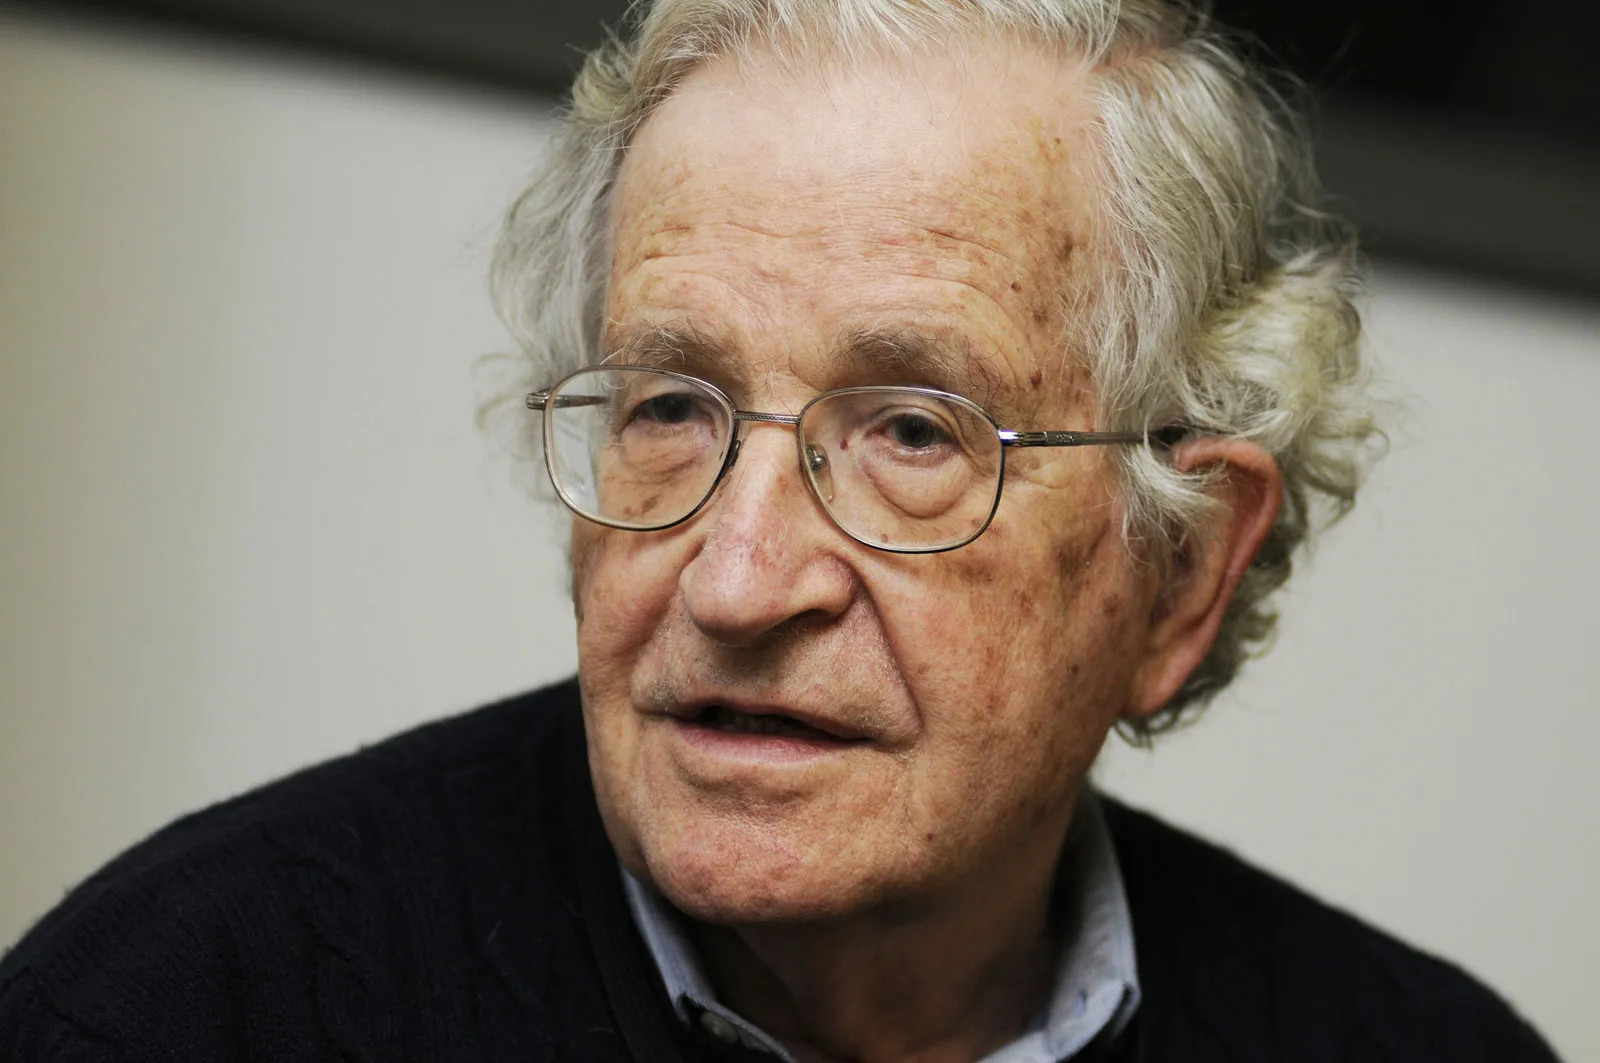
\includegraphics[width=\textwidth]{img/chomsky.jpeg}
            \end{subfigure}
            \begin{subfigure}{.4\linewidth}
                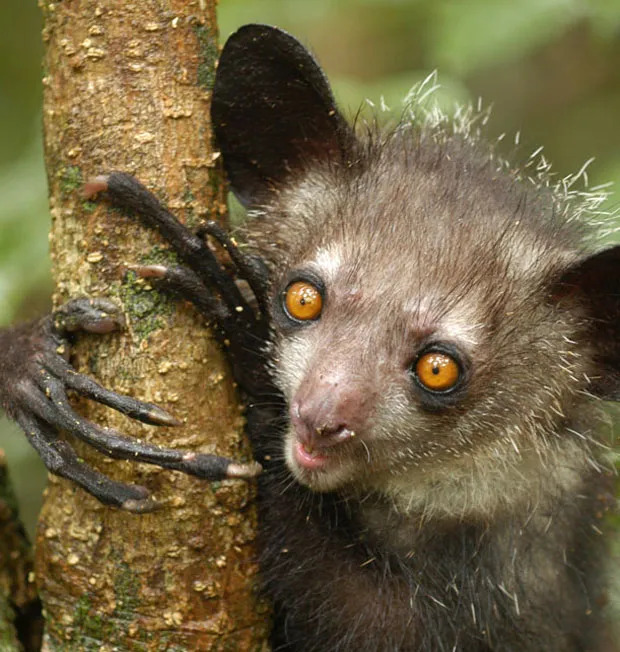
\includegraphics[width=\textwidth]{img/ayeaye.jpeg}
            \end{subfigure}
            \caption{a startling similarity.}
        \end{figure}

    \item[Different language means less intuition]
    \item[Why should machine intelligence follow behaviorism?]
    \item[But you can just program a rule]
\end{description}
is behaviorism an expressive enough framework to describe and predict AI agents' results?
to verify it, first we need to show how the basic terminology applies to AI agents. then, we will use the rich history of criticisms that have been raised against the discipline to battle-test our "implementation" of behaviorism. finally, we review why: to avoid mentalistic explanations of behavior and to have a "middle-ground theory" under which comparisons between results are fair...er.

\printbibliography


\end{document}